\Variant{04.12.2022}
\QQ{1}{$a$, $b$, $c$ — turli raqamlar bölsa, $100a+10b+c$ ning eng katta qiymatini toping.
\Opts{$897$}{$987$}{$999$}{$988$}}
\QQ{2}{Hisoblang:
\[\left(2022-\frac1{2022}\right):\frac{2021}{2022}\cdot\frac1{2023}\]
\Opts{$1$}{$2022$}{$\dfrac1{2023}$}{$2023$}}
\QQ{3}{$2$ va $3$ ga bölinmaydigan barça ikki xonali natural sonlar yiğindisini toping.
\Opts{$1620$}{$1800$}{$1960$}{$3080$}}
\QQ{4}{$A$ şahardan $B$ şaharga ikkita maşina yölga çiqdi. Birinçi maşina tezligi $v_1$, ikkinçi maşina tezligi $v_2$ ($v_1>v_2$). Birinçi maşina $B$ şaharga borib şu zahoti qaytib ikkinçi maşina bilan uçraşdi. Ikkinçi maşina bosib ötgan masofa $A$ va $B$ şaharlar orasidagi masofaning neça foizini taşkil etadi?
\Opts{$\dfrac{2v_2}{v_1+v_2}\cdot100\%$}{$\dfrac{v_2}{v_1+v_2}\cdot100\%$}{$\dfrac{2v_1}{v_1-v_2}\cdot100\%$}{$\dfrac{v_1}{v_1-v_2}\cdot100\%$}}
\QQ{5}{$3$ ta quvur berilgan. 1-quvur yolğiz özi basseynni $5$ soatda töldiradi, 2-quvur yolğiz özi basseynni $3$ soatda töldiradi, 3-quvur yolğiz özi basseynni $2$ soatda böşatadi. $3$ ta quvur bir vaqtda neça soatda basseynni töldiradi?
\Opts{$20$}{$30$}{$40$}{$15$}}
\QQ{6}{Hisoblang:
\[\sqrt[3]{\frac{12}{25}\cdot\sqrt{\frac{244}{15\cdot\left(38^2-23^2\right)}}}\]
\Opts{$0{,}8$}{$0{,}6$}{$0{,}2$}{$0{,}4$}}
\QQ{7}{Işorasi almaşinuvçi geometrik progressiyada $b_1=a-5$, $b_2=a+4$, $b_3=5a+8$ bölsa, $b_4$ ni toping.
\Opts{$\dfrac14$}{$-\dfrac14$}{$4$}{$-4$}}
\QQ{8}{Soddalaştiring:
\[\frac1{(x+y)^2}\cdot\left(\frac1{x^2}+\frac1{y^2}\right)+\frac2{(x+y)^3}\cdot\left(\frac1x+\frac1y\right)\]
\Opts{$\dfrac1{xy}$}{$\dfrac1{x^2y^2}$}{$1$}{$x+y$}}
\QQ{9}{$2x^2-5x+4=0$ tenglama neçta haqiqiy ildizga ega?
\Opts{haqiqiy ildizga ega emas}{$1$ ta}{$2$ ta}{çeksiz köp yeçimga ega}}
\QQ{10}{Hisoblang:
\[2\sin\frac{7\pi}6+\cos^2\frac{7\pi}4\]
\Opts{$-\dfrac14$}{$-\dfrac12$}{$0$}{$\dfrac12$}}
\QQ{11}{$a>5$ bölsa, $\sqrt{(3-a)^2}-\sqrt{(a-5)^2}$ ni hisoblang.
\Opts{$1$}{$-2a+8$}{$2$}{aniqlab bölmaydi}}
\QQ{12}{$\dfrac ab=4$, $\dfrac bc=10$ bölsa, $\dfrac{a^2+b^2+c^2}{ac}+\dfrac ac$ ni hisoblang.
\Opts{$81\dfrac{21}{40}$}{$82\dfrac{21}{40}$}{$80\dfrac{21}{40}$}{$81\dfrac{21}{34}$}}
\QQ{13}{Soddalaştiring:
\[\frac{2\cos\alpha+\cos3\alpha+\cos5\alpha}{\cos3\alpha+\sin\alpha\cdot\sin2\alpha}\]
\Opts{$\cos2\alpha$}{$4\cos2\alpha$}{$4\sin2\alpha$}{$\cos\alpha$}}
\QQ{14}{$3\cdot4^x+2\cdot25^x=5\cdot10^x$ tenglama neçta haqiqiy ildizga ega?
\Opts{haqiqiy ildizga ega emas}{$1$ ta}{$2$ ta}{çeksiz köp yeçimga ega}}
\QQ{15}{Toq funksiyani toping.
\Opts{$f(x)=\dfrac{\sin x+x^3}{\cos x-1}$}{$f(x)=\dfrac{\cos x+x^3}{\sin x-1}$}{$f(x)=\dfrac{\tg x+x^3}{\sin x-1}$}{$f(x)=\dfrac{\ctg x+x^2}{\cos x-1}$}}
\QQ{16}{$x^2+4x+1=2\sqrt{x^2+4x+4}$ tenglamaning haqiqiy ildizlari yiğindisini toping.
\Opts{$-4$}{$4$}{$-2$}{$-6$}}
\QQ{17}{$\bigl||2x-1|-7\bigr|\le5$ tengsizlikni qanoatlantiruvçi butun yeçimlar neçta?
\Opts{$20$ ta}{$12$ ta}{$10$ ta}{$8$ ta}}
\QQ{18}{Tengsizlikni yeçing:
\[\sqrt{4-x^2}\ge0\]
\Opts{$[-2;\,2]$}{$(-1;\,2]$}{$(-1;\,\infty)$}{$\{-2\}\cup(-1;\,2]$}}
\QQ{19}{$32^3\cdot8^{12}\cdot125^{17}$ neça xonali son?
\Opts{$52$}{$51$}{$50$}{$17$}}
\QQ{20}{Tengsizlikni yeçing:
\[\log_{\cos2x}(\sin2x)\le1\]
\Opts{$\left[\dfrac\pi8+\pi k;\,\dfrac\pi4+\pi k\right],\ k\in\mathbb Z$}{$\left[\dfrac\pi8+\pi k;\,\dfrac{5\pi}8+\pi k\right],\ k\in\mathbb Z$}{$\left[\dfrac\pi8+\pi k;\,\dfrac\pi4+\pi k\right),\ k\in\mathbb Z$}{$\left[\dfrac\pi4+2\pi k;\,\dfrac{5\pi}4+2\pi k\right),\ k\in\mathbb Z$}}
\QQ{21}{$f\bigl(g^{-1}(g(x))+1\bigr)=x^2+5x+6$ berilgan. $g^{-1}(x)$ — $g(x)$ funksiyaning teskari funksiyasi. $f(-1)$ ni toping.
\Opts{$-1$}{$2$}{$1$}{$0$}}
\QQ{22}{$f(x)=\sin^25x-|\cos2x+x|$ funksiya berilgan. $f'\left(-\dfrac\pi6\right)$ ni toping.
\Opts{$\dfrac{7\sqrt3+2}2$}{$-\sqrt3+1$}{$\dfrac{3\sqrt3+4}2$}{$\dfrac{3\sqrt3-2}2$}}
\QQ{23}{Çizmadagi maʼlumotlardan foydalanib $x$ ni toping ($AB\parallel EF$).
\qfig{\begin{tikzpicture}[scale=0.3,font=\small]
\coordinate (A) at (0,0); \coordinate (C) at (20,0); \coordinate (B) at (10.706,11.890); \coordinate (F) at (5,0); \coordinate (E) at (13.03,8.918);
\draw (A)--(B)--(C)--cycle; \draw (F)--(E);
\node[left] at (A) {$A$}; \node[above] at (B) {$B$}; \node[right] at (C) {$C$}; \node[below] at (F) {$F$}; \node[above right] at (E) {$E$};
\node[above left] at ($(A)!0.5!(B)$) {$16$}; \node[above left] at ($(F)!0.5!(E)$) {$12$}; \node[above] at (12.5,0) {$x$};
\draw[{Stealth[length=3pt]}-{Stealth[length=3pt]}] (0,-1.6)--(20,-1.6); \draw (0,-1.1)--(0,-2.1); \draw (20,-1.1)--(20,-2.1); \node[fill=white,inner sep=1pt] at (10,-1.6) {$20$};
\end{tikzpicture}}
\Opts{$10$}{$15$}{$12$}{$8$}}
\QQ{24}{Tekislikka ikkita $AB$ va $BC$ oğma va $BH$ perpendikulyar tuşirilgan. Bunda $BH=HC$, $AB=2HC$, $\angle AHC=90^\circ$ bölsa, $\cos\angle BAC$ ni toping.
\Opts{$\dfrac34$}{$\dfrac35$}{$\dfrac13$}{$\dfrac12$}}
\QQ{25}{Tomoni $4$ ga teng bölgan kvadratga doira içki çizilgan. Doiraning yuzini toping.
\Opts{$16\pi$}{$\pi$}{$2\pi$}{$4\pi$}}
\QQ{26}{$ABC$ uçburçakda $\angle BAC=90^\circ$ va $\angle BCA=30^\circ$ bölib, $BD$ bissektrisa $2\sqrt2$ ga teng bölsa, $ABC$ uçburçak yuzini toping.
\Opts{$2\sqrt3$}{$2\sqrt2$}{$3\sqrt2$}{$3\sqrt3$}}
\QQ{27}{Diagonallari soni tomonlar sonidan $6$ marta köp bölgan köpburçakning içki burçaklari yiğindisini toping.
\Opts{$2700^\circ$}{$1800^\circ$}{$2340^\circ$}{$2400^\circ$}}
\QQ{28}{Rombning katta diagonali $10\sqrt{4+2\sqrt2}$ ga, ötkir burçagi $45^\circ$ bölsa, diagonallari kesişiş nuqtasidan tomonlarigaça bölgan eng qisqa masofalar yiğindisini toping.
\Opts{$10$}{$20$}{$15$}{$25$}}
\QQ{29}{Hisoblang:
\[\int\limits_{-3}^42x^2\,|2x|\,dx\]
\Opts{$187$}{$175$}{$337$}{$222$}}
\QQ{30}{$ABC$ uçburçakning yuzi $60$ ga teng. $\overrightarrow{BE}=\overrightarrow{AB}$ bölsa, $AEC$ uçburçakning yuzini toping.
\Opts{$120$}{$90$}{$60$}{$30$}}
\QQ{31}{$(A\cap B)\cup(A\cup B)'$ ning elementlari sonini toping.
\qfig{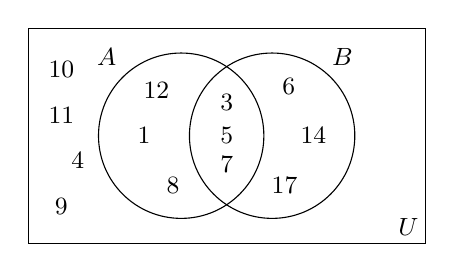
\begin{tikzpicture}[scale=1.05,font=\small]
\draw (-2.4,-1.3) rectangle (2.4,1.3); \draw (-0.55,0) circle (1); \draw (0.55,0) circle (1);
\node at (-1.45,0.95) {$A$}; \node at (1.4,0.95) {$B$}; \node at (2.2,-1.1) {$U$};
\foreach \t/\x/\y in {10/-2.0/0.8,11/-2.0/0.25,4/-1.8/-0.3,9/-2.0/-0.85,12/-0.85/0.55,1/-1.0/0,8/-0.65/-0.6,3/0/0.4,5/0/0,7/0/-0.35,6/0.75/0.6,14/1.05/0,17/0.7/-0.6} \node at (\x,\y) {$\t$};
\end{tikzpicture}}
\Opts{$5$}{$7$}{$6$}{$9$}}
\QQ{32}{Merganning nişonga tekkaziş ehtimoli $0{,}8$ ga teng. $5$ marta öq uzilgan. Dastlab otilgan $3$ ta öq tegib, keyingi $2$ ta otilgan öq tegmaslik ehtimolini toping.
\Opts{$2^{10}\cdot10^{-6}$}{$2^{11}\cdot10^{-5}$}{$2^{11}\cdot10^{-6}$}{$2^{10}\cdot10^{-5}$}}
\QQ{33}{\Moslash{Muntazam oltiburçakli piramidaga şar içki çizilgan. Şar içiga eng katta hajmli konus içki çizilgan. Piramida asosining tomoni $6$ ga, yon yoği asos tekisligi bilan $60^\circ$ burçak taşkil etadi. ($\pi\approx3$ deb oling.)}{A) $162\sqrt3$\par B) $108$\par C) $32$\par D) $81$\par E) $81\sqrt3$\par F) $27$}{Piramida hajmini toping.}{Şar hajmini toping.}{Konus hajmini toping.}}
\QQ{36}{$\dfrac{6x-k}{x-1}=\dfrac{3x+k}{x+1}$ tenglama berilgan.
\AB{Tenglama bitta ildizga ega böladigan $k$ ning eng katta qiymatini toping.}{Tenglama bitta ildizga ega böladigan $k$ ning barça qiymatlari yiğindisini toping.}}
\QQ{37}{$3\left(\log_2\sin x\right)^2+\log_2(1-\cos2x)=2$ tenglamani yeçing.
\AB{Tenglamaning eng kiçik musbat ildizini toping.}{Tenglama $\left(-\dfrac\pi2;\,\dfrac{5\pi}2\right)$ oraliqda neçta ildizga ega?}}
\QQ{38}{$g(x)=kx+l$ va $f(x)=ax^2+bx+c$ funksiyalar grafiklari berilgan. Grafikdan foydalanib, quyidagilarni hisoblang.
\qfig{\begin{tikzpicture}[scale=0.42,font=\small]
\draw[-{Stealth[length=4pt]}] (-3.5,0)--(7.5,0) node[right] {$x$}; \draw[-{Stealth[length=4pt]}] (0,-2.2)--(0,7.5) node[left] {$y$};
\draw[thick,domain=-2.6:4.6,samples=80] plot (\x,{-0.5*\x*\x+\x+4}); \draw[thick] (-1,7)--(7,-1); \draw[dashed] (2,0)--(2,4);
\fill (0,4) circle (3pt); \fill (0,6) circle (3pt); \fill (2,4) circle (3pt);
\node[left] at (0,4.3) {$4$}; \node[left] at (0,6.2) {$6$}; \node[below left] at (-2,0) {$-2$}; \node[below] at (2,0) {$2$}; \node[below left] at (6,0) {$6$};
\node[left] at (-1.8,2.4) {$f(x)$}; \node[right] at (4,3) {$g(x)$};
\end{tikzpicture}}
\AB{$f'(2)$ ni hisoblang.}{$f'\left(\dfrac1a\right)-5f'\left(\dfrac1b\right)+2f'\left(\dfrac1c\right)$ ni hisoblang.}}
\QQ{39}{$f(x)=x^4-2x^3+2x^2-2x+1$ bölsa,
\AB{$f\left(1+\sqrt2\right)+f\left(1-\sqrt2\right)$ ni hisoblang.}{$f(x)=0$ tenglama neçta turli haqiqiy ildizga ega?}}
\QQ{40}{Rasmda $f(x)=ax^2+bx+c$ parabola va $g(x)=kx+l$ töğri çiziq grafiklari tasvirlangan. $(-2;\,0)$ va $(x_0;\,y_0)$ nuqtalar parabola va töğri çiziq kesişgan nuqtalar bölsa,
\qfig{\begin{tikzpicture}[xscale=0.4,yscale=0.32,font=\small]
\fill[qfill] plot[domain=-2:8,samples=60] (\x,{0.2*(\x+2)*(\x-5)})--cycle;
\draw[-{Stealth[length=4pt]}] (-3.5,0)--(10.5,0) node[right] {$x$}; \draw[-{Stealth[length=4pt]}] (0,-4.2)--(0,9.5) node[left] {$y$};
\draw[thick,domain=-2.6:8.6,samples=80] plot (\x,{0.2*(\x+2)*(\x-5)}); \draw[thick] (-3.3,-0.78)--(9.5,6.9);
\foreach \p in {(-2,0),(0,1.2),(0,-2),(5,0),(8,6)} \fill \p circle (4pt);
\node[above left] at (-2,0) {\scriptsize$(-2;\,0)$}; \node[above right] at (0,1.2) {\scriptsize$(0;\,1{,}2)$}; \node[left] at (0,-2.2) {\scriptsize$(0;\,-2)$};
\node[below right] at (5,0) {\scriptsize$(5;\,0)$}; \node[right] at (8.1,5.8) {\scriptsize$(x_0;\,y_0)$};
\end{tikzpicture}}
\AB{$x_0+y_0$ ni hisoblang.}{Böyalgan sohaning yuzini toping.}}
\QQ{41}{$ABC$ uçburçakda $AB=7$, $BC=10$, $AC=15$ ga teng. Uçburçakka ikkita aylana şunday içki çizilganki, $R$ radiusli aylana uçburçak tomonlariga, $r$ radiusli aylana esa $AC$, $BC$ va $R$ radiusli aylanaga urinadi.
\qfig{\begin{tikzpicture}[scale=0.5,font=\small]
\coordinate (A) at (0,0); \coordinate (C) at (15,0); \coordinate (B) at (5.8,3.919); \coordinate (I) at (6,1.837); \coordinate (J) at (9,1.2247);
\draw (A)--(B)--(C)--cycle; \draw (I) circle (1.837); \draw (J) circle (1.2247); \fill (I) circle (2.5pt); \fill (J) circle (2.5pt);
\draw (I)--($(I)+(60:1.837)$); \draw (J)--($(J)+(60:1.2247)$); \node at (6.75,2.4) {\scriptsize$R$}; \node at (9.55,1.6) {\scriptsize$r$};
\node[left] at (A) {$A$}; \node[above] at (B) {$B$}; \node[right] at (C) {$C$};
\node[above left] at ($(A)!0.5!(B)$) {$7$}; \node[above right] at ($(B)!0.6!(C)$) {$10$}; \node[below] at (7.5,0) {$15$};
\end{tikzpicture}}
\AB{$R$ ni toping.}{$r$ ni toping.}}
\QQ{42}{Quyidagi çizmada yuzi $42$ ga teng bölgan $ABCD$ trapetsiya tasvirlangan. Trapetsiyaning $BC$ yon tomonidan $K$ va $L$ nuqtalar olingan. $\dfrac{CL}{LK}=\dfrac32$, $\dfrac{KB}{LK}=2$ va $\dfrac{DC}{AB}=\dfrac59$ bölsa,
\qfig{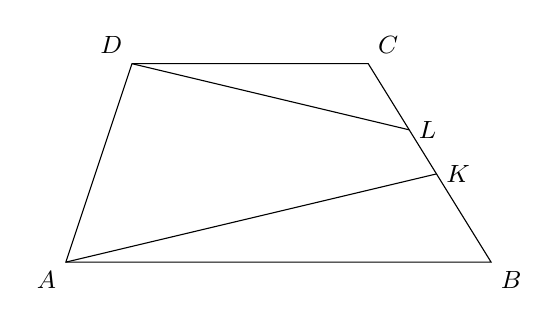
\begin{tikzpicture}[scale=0.6,font=\small]
\coordinate (A) at (0,0); \coordinate (B) at (9,0); \coordinate (C) at (6.4,4.2); \coordinate (D) at (1.4,4.2); \coordinate (L) at (7.267,2.8); \coordinate (K) at (7.844,1.867);
\draw (A)--(B)--(C)--(D)--cycle; \draw (A)--(K); \draw (D)--(L);
\node[below left] at (A) {$A$}; \node[below right] at (B) {$B$}; \node[above right] at (C) {$C$}; \node[above left] at (D) {$D$}; \node[right] at (L) {$L$}; \node[right] at (K) {$K$};
\end{tikzpicture}}
\AB{$AKB$ uçburçakning yuzini toping.}{$AKLD$ törtburçakning yuzini toping.}}
\QQ{43}{Rasmda aylananing $\dfrac14$ qismi tasvirlangan. $AC=AB=R$ — aylana radiusi, $CD=1$, $BD=3\sqrt2$ bölsa,
\qfig{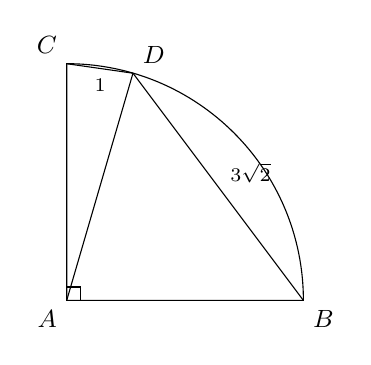
\begin{tikzpicture}[scale=0.85,font=\small]
\coordinate (A) at (0,0); \coordinate (B) at (3.536,0); \coordinate (C) at (0,3.536); \coordinate (D) at (0.99,3.394);
\draw (A)--(B) arc (0:90:3.536)--cycle; \draw (C)--(D)--(B); \draw (A)--(D); \draw (0,0.2)--(0.2,0.2)--(0.2,0);
\node[below left] at (A) {$A$}; \node[below right] at (B) {$B$}; \node[above left] at (C) {$C$}; \node[above right] at (D) {$D$};
\node[below] at (0.5,3.45) {\scriptsize$1$}; \node[right] at (2.3,1.9) {\scriptsize$3\sqrt2$};
\end{tikzpicture}}
\AB{$\sin\angle CAD$ ni toping.}{$CAD$ uçburçakning yuzini toping.}}
\QQ{44}{Silindrga oktaedr içki çizilgan. Oktaedrning hajmi $36$ ga teng.
\AB{Oktaedrning qirrasini toping.}{Silindr hajmini toping.}}
\QQ{45}{Tomonlari $2$ va $10$ ga teng bölgan töğri törtburçakli metalldan asoslari ikkita doira va yon sirti qirqib olib, silindr hosil qilindi ($\pi\approx3$ deb oling).
\qfig{\begin{tikzpicture}[scale=0.55,font=\small]
\fill[qfill] (0,0) rectangle (10,2); \draw (0,0) rectangle (10,2); \node[left] at (0,1) {$2$}; \node[below] at (5,0) {$10$};
\end{tikzpicture}}
\AB{Eng kam çiqindi çiqarib silindr yasalsa, uning hajmini toping.}{Silindr yasaşdan hosil bölgan çiqindi metallning neça foizini taşkil etadi?}}
\Javoblar{B A A A B D A B A B C B B C A A C A A C D A B A D D C B C A B B A B C}{\OK{36}{$6$}{$13{,}5$}\OK{37}{$\dfrac\pi6$}{$3$}\OK{38}{$-1$}{$4{,}5$}\OK{39}{$16$}{$1$}\OK{40}{$14$}{$\dfrac{100}3$}\OK{41}{$\dfrac{3\sqrt6}4$}{$\dfrac{\sqrt6}2$}\OK{42}{$12$}{$25$}\OK{43}{$\dfrac7{25}$}{$\dfrac74$}\OK{44}{$3\sqrt2$}{$54\pi$}\OK{45}{$6$}{$10\%$}}
